% Conteudo do capitulo
%1- Razoes fisicas para se ter o ATLAS UPGRADE 
%2- Porque a melhor escolha para o upgrade e o LGAD
%3- Importacia cientifica do LGAD
%4- Introducao ao LGAD
%5- Proposta do projeto
%6- Alguns detalhes sobre o escopo do projeto
%7- Importancia para o grupo 
\chapter{Introdução}

% 1 - Razoes físicas para se ter o ATLAS UPGRADE 
Para o experimento ATLAS, o desafio experimental é reconstruir partículas na região de rapidez frontal, produzidas na interação inicial de modo a associá-las corretamente com o vértice onde foram originadas, em um regime de altas taxas de colisão. Para solucionar esse desafio, um novo sistema de detecção frontal, denominado HGTD ({\it High Granularity Timing Detector}), está sendo desenvolvido - com base nos sensores LGAD ({\it Low Gain Avalanche Detector}) - para fornecer uma medida precisa de tempo, com o objetivo de diminuir os efeitos do {\it pile-up} dos eventos. 

Em maiores detalhes, de modo geral a capacidade de associar as trajetórias ao vértice primário depende da precisão na determinação do parâmetro de impacto longitudinal. Enquanto que para trajetórias centrais com pseudo-rapidez no intervalo $\eta<1.5$, o parâmetro de impacto longitudinal é pequeno e determinado com grande precisão, para trajetórias frontais com $\eta>2.5$ o parâmetro de impacto cresce rapidamente atingindo valores da ordem de milímetros \cite{tdr}. Esse é um comportamento perfeitamente explicado pelo fato delas tornarem se mais colineares com a linha do feixe, o que associado à segmentação do detector dificulta a extrapolação das trajetórias para a posição do vértice da colisão, resultando em grandes valores obtidos para o parâmetro de impacto longitudinal.

Desse modo, devido à baixa resolução presente na medida da proximidade longitudinal ao vértice primário, trajetórias frontais são mais difíceis de associar de forma não ambígua com o vértice do evento. Devido a isso, e para preservar a excelente resolução obtida para as trajetórias centrais, com a construção e utilização do HGTD o experimento ATLAS será capaz de associar com grande precisão trajetórias frontais ao vértice da colisão para eventos que acontecem muito próximos no espaço, entretanto em instante de tempo distintos. Utilizando a informação do tempo em que as colisões acontecem - fornecida pelo HGTD - será possível identificar quais trajetórias frontais pertencem a um determinado vértice rejeitando trajetórias originadas em outras interações espacialmente próximas ao vértice em questão. 

Por conseguinte, com o aumento significativo da eficiência na medida de partículas frontais, através do uso do HGTD, será possível medir com precisão a luminosidade do feixe, a qual é uma medida crítica para a determinação da seção de choque da produção de partículas em diversas analises físicas, além de  permitir a reconstrução de jatos de partículas com grande precisão. A melhoria na capacidade de reconstrução de jatos - que será obtida com o HGTD - aumentará a sensibilidade do experimento, permitindo explorar observáveis antes não explorados devido aos limites experimentais.
Em seguida, como ilustra a Fig. \ref{hgtd}, o HGTD foi concebido para ser instalado na região frontal do experimento, em ambos os lados a uma distancia de $3.5m$ do ponto de interação do feixe, região a qual está localizada após o volume do ATLAS {\it Inner Tracker} (ITk) \cite{tdr}. 

\begin{figure} 
    \centering
    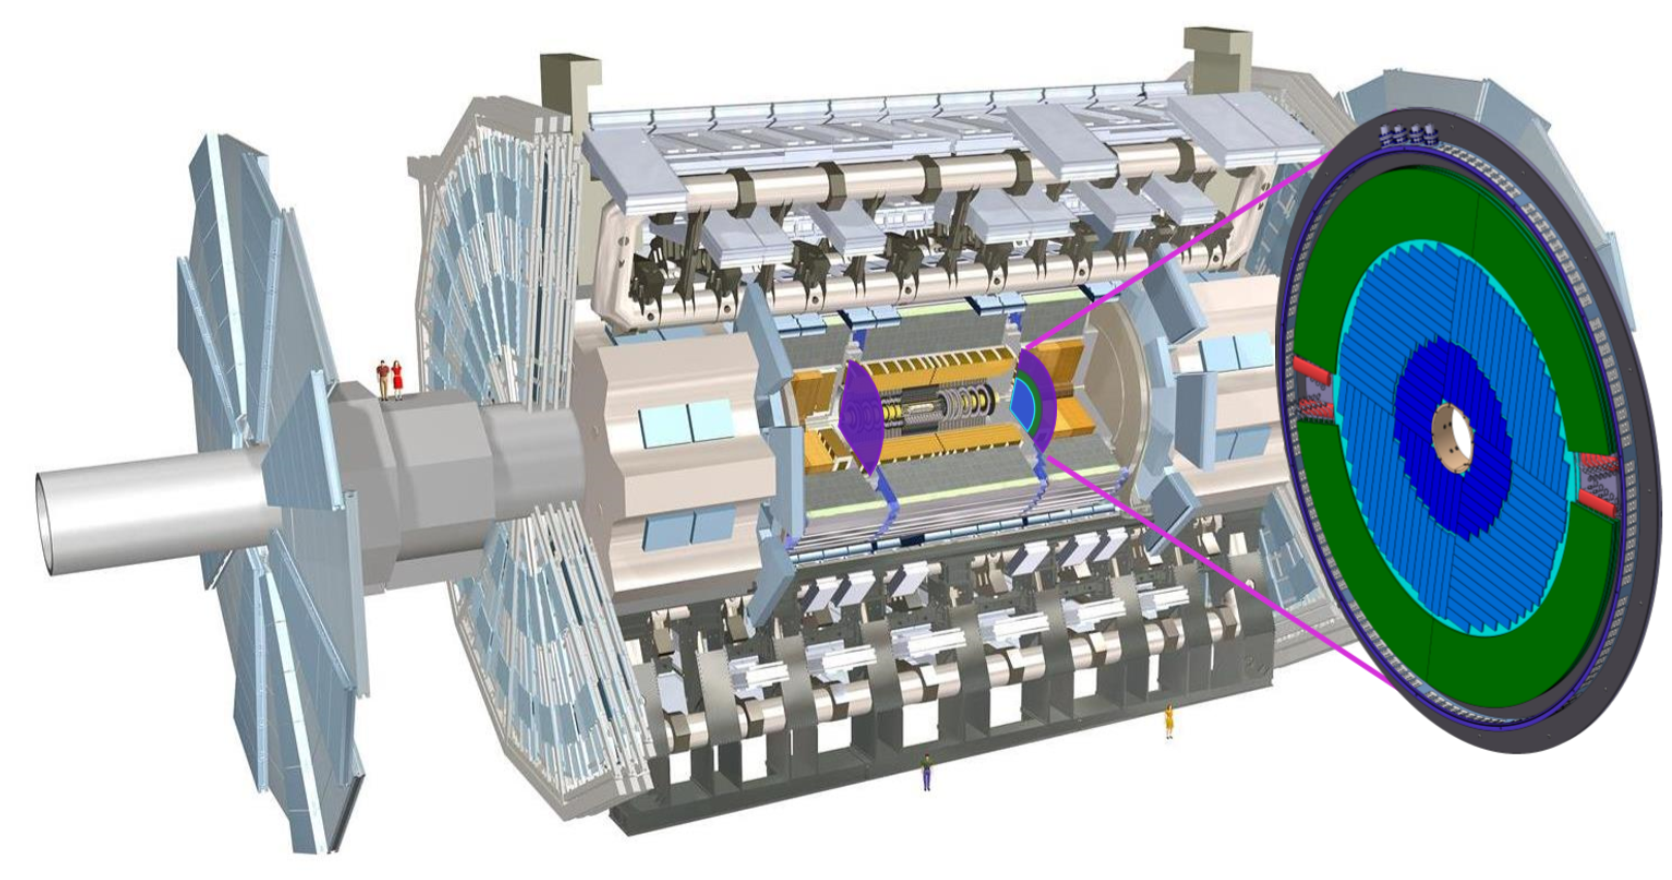
\includegraphics[width=15.0cm]{assets/ATLAS_HGTD.png}
    \caption{ Figura mostrando no detalhe mostra a posição onde o HGTD será instalado. Figura também mostra o experimento ATLAS e os seus vários sistemas.}
    \label{hgtd}
\end{figure}

%2-  Porque a melhor escolha para o upgrade e o LGAD
Neste ponto cabe destacar que os sensores LGAD foram adotados como base tecnológica para a construção do HGTD por apresentarem excelentes características com respeito ao compromisso entre ganho e resolução temporal \cite{tdr,JIN_LGAD,NIMA_LGAD,NIMA_LGAD_I,NIMA_LGAD_II,NIMA_LGAD_III}. A Fig. \ref{timeresolution} mostra quatro conjuntos de dados medidos - utilizando os primeiros protótipos do sensor irradiados em  diferentes valores de fluência de nêutrons - onde é possível observar a dependência da resolução em tempo em função de seu ganho. De acordo com os dados, eles demonstram que é possível atingir resolução em tempo menores que 30ps com valores moderados de ganho.   

\begin{figure} 
    \centering
    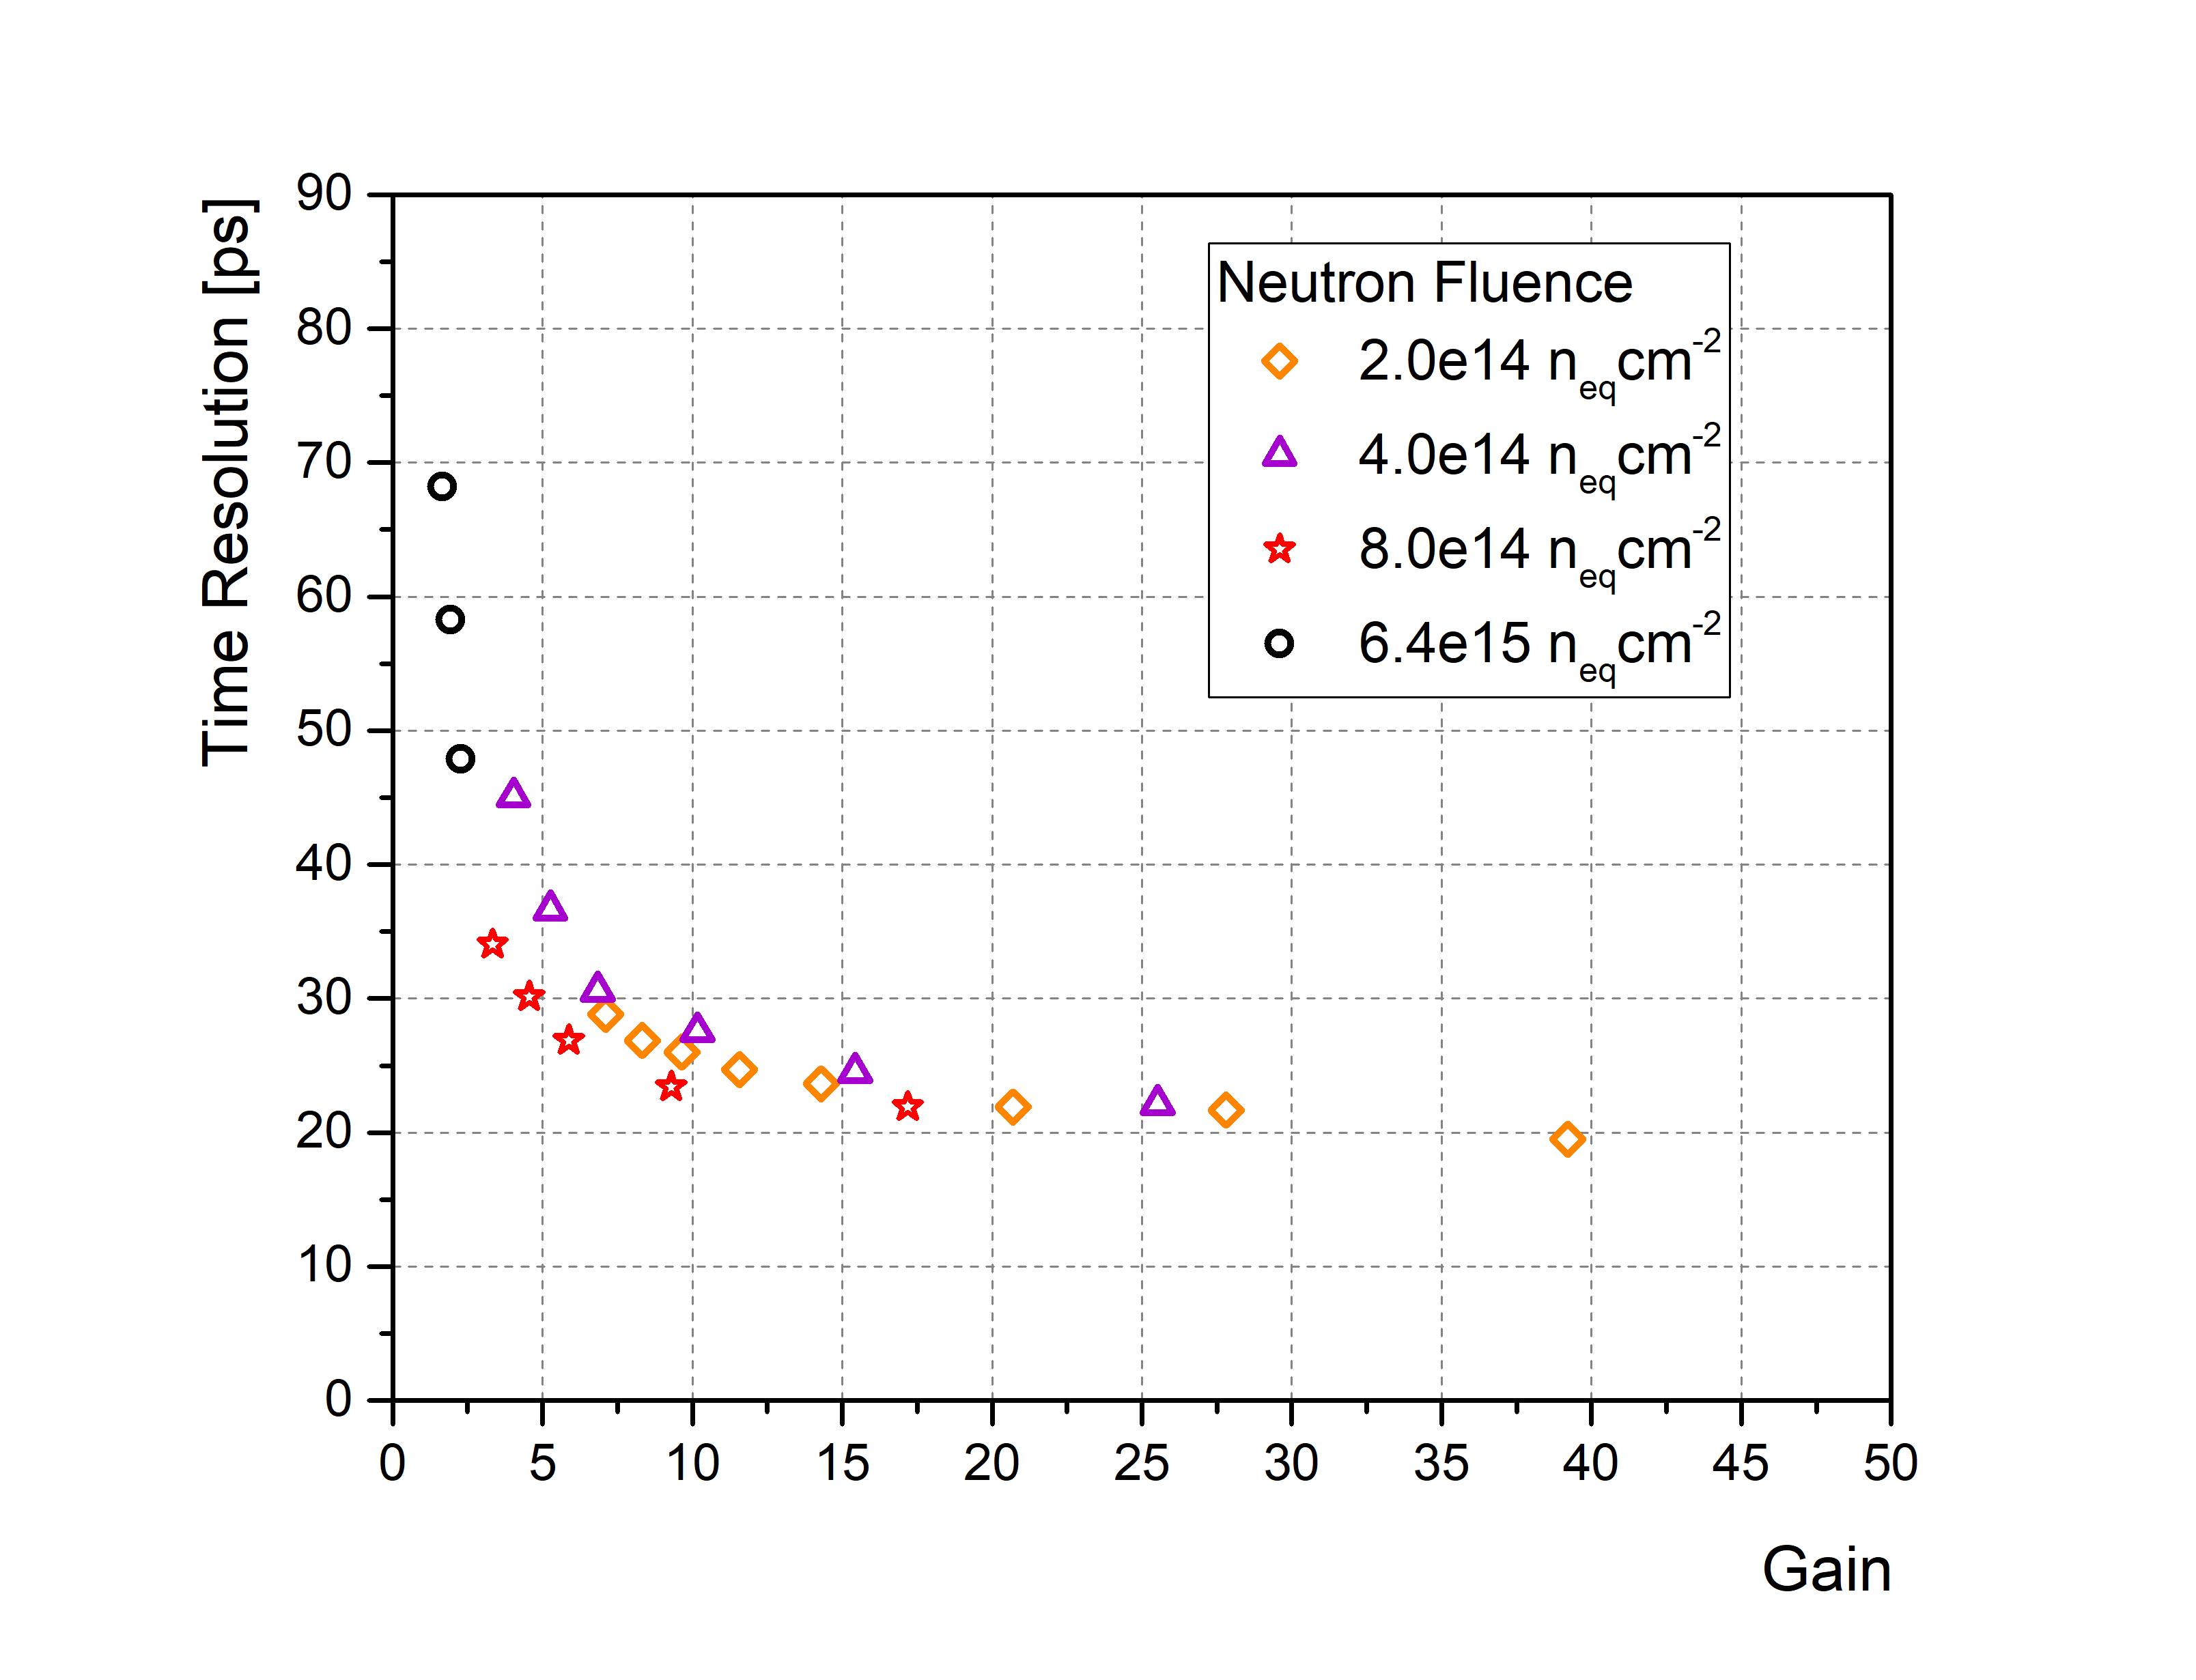
\includegraphics[width=12.0cm]{assets/timeresolution_vs_gain.png}
    \caption{ Gráfico mostrando a resolução temporal em função do ganho do LGAD. Dados retirados da referência \cite{tdr}.}
    \label{timeresolution}
\end{figure}

% 3- Importância cientifica do LGAD
Em maiores detalhes, detectores semicondutores de resposta rápida do tipo LGAD é um sensor introduzido recentemente no escopo do desenvolvimento de sensores semicondutores \cite{JIN_LGAD,NIMA_LGAD}, cuja capacidade de produzir sinais em intervalos de tempo muito curtos possibilita a medida de eventos produzidos em colisões próton-próton nos experimentos de física de altas energias, em intervalos de tempo da ordem de pico segundos. 

Além da resposta rápida à incidência de radiação, esse tipo de sensor possui ganho intrínseco devido ao perfil de dopagem empregado no material semicondutor, o que torna possível amplificar o sinal produzido e dessa forma operá-lo em modo de avalanche de carga \cite{JIN_LGAD,NIMA_LGAD,NIMA_LGAD_I,NIMA_LGAD_II,NIMA_LGAD_III}. Essas características demonstram a importância dessa tecnologia para o desenvolvimento da próxima geração de sensores semicondutores para aplicações que requerem altas taxas de contagem e ganho moderado.

% 4- Introdução ao LGAD
Os primeiros sensores baseados em LGAD foram desenvolvidos no Centro Nacional de Microeletrônica (CNM) em Barcelona e posteriormente pela colaboração RD50-CERN \cite{tdr}, a qual é uma colaboração localizada no CERN que visa desenvolver detectores semicondutores para aplicações com feixes de alta intensidade.% Além disso, o RD50 promove o surgimento de novas aplicações e inovações através do desenvolvimento de ferramentas e da consolidação do conhecimento e dos fenômenos físicos relacionados com sensores semicondutores. 

Em maiores detalhes, LGAD são sensores semicondutores planos com ganho intrínseco como ilustra a Fig. \ref{lgad}. O ganho do sensor é determinado pela quantidade de dopante implantado na matriz de silício formando a camada de multiplicação. Como mostra a Fig. \ref{lgad}, sua arquitetura é composta de uma camada de material semicondutor do tipo n sobre uma camada do tipo p, com a adição de uma camada altamente dopada do tipo p localizada entre a junção n-p, cuja função é criar um alto campo elétrico responsável por produzir a avalanche das cargas e amplificar o sinal elétrico. Dessa forma, quando uma partícula atravessa a região sensível do detector, elétrons e lacunas são criados produzindo uma corrente inicial. Os elétrons ao atingirem a região de amplificação produzem novos pares elétron lacuna sendo desse modo multiplicados em um processo de avalanche, produzindo uma corrente de 10 a 30 vezes maior do que a produzida em um diodo padrão \cite{JIN_LGAD,NIMA_LGAD_III}. 

\begin{figure}
    \centering
    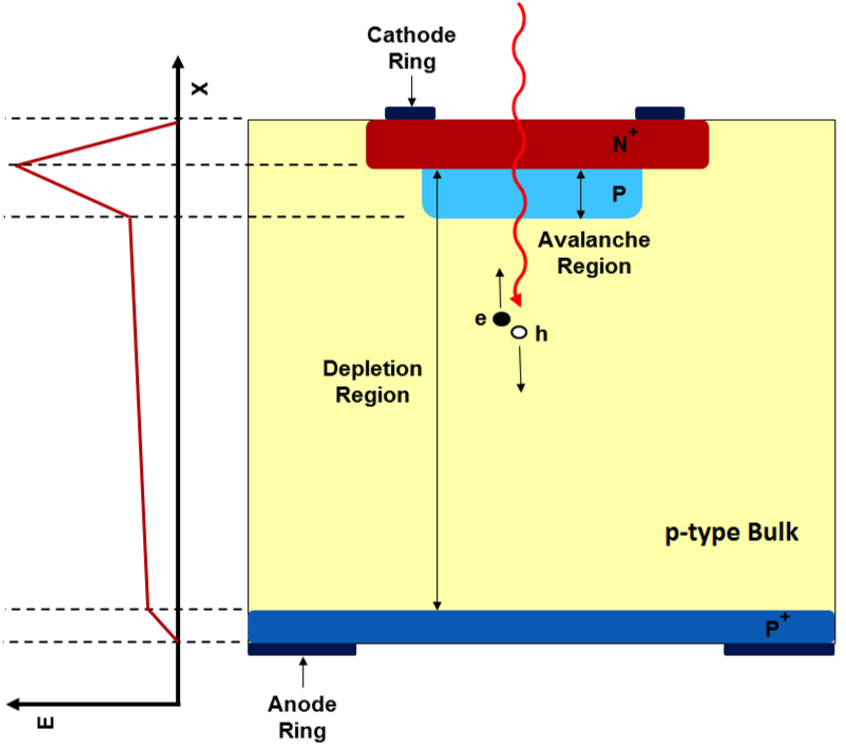
\includegraphics[width=7.0cm]{assets/lgad.png}
    \caption{Figura mostrando a estrutura esquemática de um sensor LGAD.}
    \label{lgad}
\end{figure}

% 5 - PROPOSTA DO PROJETO
A vista disso, um dos propósitos deste projeto é desenvolver técnicas e metodologias necessárias para a caracterização física de sensores semicondutores do tipo LGAD. Neste escopo a colaboração com o experimento ATLAS no CERN será fundamental pois irá servir de ponte para a troca de conhecimento e experiência permitindo introduzir esse tipo de tecnologia no IFUSP.

%-------------------- 4.1 colocar algo mais com respeito ao btagging e reconstrucao de jatos 
% para a realizacao deste detector sera empregado sensore LGAD....

% 6- Alguns detalhes sobre o escopo do projeto
Com isso em mente, neste projeto de pesquisa é proposto o desenvolvimento de atividades focadas na pesquisa e desenvolvimento dos sensores semicondutores do tipo LGAD com o objetivo de optimizar sua característica para utilização no HGTD do experimento ATLAS. A consolidação desse tipo de sensores oferece um grande desafio em termos de pesquisa e desenvolvimento na área de sensores semicondutores, com potencial de aplicação em diversas áreas da física e tecnologia em geral. 

O projeto será composto de várias etapas. Inicialmente pretende-se consolidar as técnicas necessárias para a caracterização dos sensores. Neste processo o pesquisador responsável e colaboradores irão estabelecer o métodos experimentais para a caracterização das propriedades físicas dos sensores. Nesta estágio, o pesquisador será responsável por montar e certificar os arranjos experimentais, desenhar e construir as parte necessárias para os mesmos, além de automatizar o processo de tomada de dados. Por fim, a comparação direta com resultados obtidos em outros centros de pesquisa dentro da colaboração ATLAS será feita para garantir a qualidade dos resultados obtidos e acelerar a consolidação dessa etapa.  
Uma vez que a primeira etapa seja concluída, sensores LGAD serão irradiados no reator multipropósito localizado no IPEN, o qual possui uma elevada fluência de nêutrons, i.e ordem de 1e16$n_{eq}cm{^{-2}}$ \cite{IPEN_REATOR}, além de um difratômetro de nêutrons denominado AURORA \cite{IPEN_AURORA}, instalado na parte externa do reator, o qual oferece grande flexibilidade para a irradiação de dispositivos. Em seguida os sensores serão caracterizados no setup previamente estabelecido com o objetivo de estudar o comportamento do ganho e resolução em tempo do sensor em função da fluência das partículas atravessando o volume sensível do detector. Essa etapa é fundamental para compreender os mecanismos associados à física do dano radioativo em sensores semicondutores e por conseguinte propor melhorias para a próxima geração de sensores. 
Neste ponto cabe destacar que as metodologias e técnicas desenvolvidas na pesquisa de novas tecnologias que aumentem a resistência dos sensores ao dano radioativo, são extremamente importantes do ponto de vista científico e tecnológico, uma vez que possibilitarão a geração de conhecimento com respeito aos efeitos físicos da radiação em materiais semicondutores dopados ainda não bem conhecidos \cite{tdr,JIN_LGAD,NIMA_LGAD}. %Neste âmbito os processos e métodos desenvolvidos na pesquisa poderão ser convertidos na produção de patentes. 
Em seguida com base nos dados coletados nesta fase de teste dos protótipos, será possível estabelecer com grande precisão as especificações que melhor atendem as necessidades do experimento ATLAS. 

%Uma vez optimizados, a solução definida será produzida em larga escala, e neste ponto o grupo fará parte do esforço em conjunto com o experimento ATLAS para qualificar os sensores que serão empregados na construção do HGTD. Essa etapa é fundamental para o exercício dos métodos desenvolvidos nas etapas anteriores bem como para a consolidação da importância do grupo de pesquisa HEPIC na esfera da colaboração ATLAS.

%-- estará contato com o Laboratório de novos materiais semicondutores da USP
Paralelamente, no âmbito nacional, através da coloração com o Laboratório de Sistemas Integráveis (LSI) da Escola Politécnica da USP - colaboração essa previamente estabelecida em projetos anteriores executados com o HEPIC \cite{ALICEUP,ref1} - será possível, através da transferência de know how, produzir sensores LGAD com o objetivo de melhorar a sua tecnologia e explorar o seu grande potencial para aplicações em outras áreas da ciência. Nessa frente de pesquisa, o pesquisador responsável irá gerenciar as tecnologias e recursos técnicos disponíveis no LSI com o objetivo de obter os melhores resultados para a produção do LGAD.  

% 6 - APLICACOES PARA A INDUSTRIA
%Ainda no ambito nacional, pretende se fazer um esforço ...

% 7 - Importancia para o grupo
Por fim, é importante destacar que a implantação dessa linha de pesquisa no HEPIC será de extrema importância para projetos futuros envolvendo sensores semicondutores. Atualmente o grupo conta com excelentes ferramentas na área de instrumentação para física nuclear e de partículas reconhecida internacionalmente, e adquirida por meio da execução de projetos em colaborações internacionais, como por exemplo o chip SAMPA focada na tecnologia de detectores gasosos \cite{ref1}. Isso somado à experiência do pesquisador responsável adquirida na execução de pesquisa e desenvolvimento no âmbito do projeto de upgrade do TPC do ALICE \cite{tpcNIM,discharge_paper,GSI_REPO}, tornará possível a transferência total de tecnologia relacionada com sensores semicondutores de alta performance para o HEPIC, bem como a geração de novas tecnologias e aplicações que poderão estabelecer o grupo como um protagonista internacional.

\renewcommand{\cleardoublepage}{}
\renewcommand{\clearpage}{}